\documentclass{article} 
\usepackage{amsmath} 
\usepackage{amssymb} 
\usepackage{amsthm} 
\usepackage[margin=0.2in]{geometry} 
\usepackage{hyperref} 
\usepackage{physics} 
\usepackage{tikz} 
\usepackage{mathtools}
\mathtoolsset{showonlyrefs} 
\theoremstyle{definition} 
\newtheorem{theorem}{Theorem}[section] 
\newtheorem{corollary}{Corollary}[theorem] 
\newtheorem{lemma}[theorem]{Lemma} 
\newtheorem{definition}{Definition}[section] 

\author{Connor Duncan}
\date{\today}

\title{notes-09-18-2019}
\begin{document}
\abstract{A single document copy of these notes, as well as a mirror of every note, can be found at \url{connorduncan.xyz/notes}}
\subsubsection{Relativistic Corrections to the Atom (Guest: Prof. Mike Zaletel)} Hydrogen atom hamiltonian \begin{equation} \hat H=\hat H_0+\hat H_k+\hat H_{s.o.}+\hat H_D \end{equation} where $H_0$ is the usual hamiltonian, $H_k$ contains corrections gained by inclusion of $\hat p^4$, $\hat H_{s.o.}$ is $\vec{L}\cdot\vec{S}$, or the spin orbit coupling term, and $\hat H_D$ is the ``Darwin'' component. \begin{center} 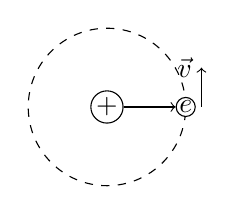
\begin{tikzpicture} \node (+) at (0,0) [draw, circle, inner sep=0.5pt] {$+$}; \draw[dashed] (0,0) ellipse (1); \node (e) at (1,0) [draw, fill=white, circle, inner sep=0.2pt] {$e$}; \draw[->] (+) -- (e); \draw[->] (1.2,0)--(1.2,.5) node[anchor=east] {$\vec{v}$}; \end{tikzpicture} \end{center} If we switch to the frame of our electron, the proton should move with velocity $-\vec{v}$. Let the charge of the proton be $Z$, so we get, in CGS units that our magnetic field should be \begin{equation} \vec{B}=\frac{-Ze\vec{v}\times\vec{r}}{cr^3} \end{equation} Since the electron carries a spin, we want \begin{equation} \hat H_{so}=-\vec{mu}\cdot\vec{B} \end{equation} We're gonna be off by a factor of 2, but that's because we aren't using the dirac equation to find solutions here. Moving on with that in mind, we write that \begin{equation} \vec{\mu}=g\mu_B\vec{S} \end{equation} so the spin orbit coupling becomes \begin{equation} \frac{Ze^2}{m_e^2c^2r^3}\vec{S}\cdot\vec{L} \end{equation} Remember, we have the factor of two though, so the actual result should be \begin{equation} \frac{Ze^2}{2m_e^2c^2r^3}\vec{S}\cdot\vec{L} \end{equation} Our base hamiltonian has eigenspectra $H_0:\ket{n,\ell,m}$. When we go to spin, we get $\ket{n,\ell,m}\otimes\ket{Z=\pm\frac{1}{2}}$. This is gonna yeet our $SO(3)$ symmetry in $\ell,Z$, which is sad! But if we want to make this easier, we should take \begin{equation} \vec{J}=\vec{L}+\vec{S} \end{equation} We should note the following properties \begin{align} [\vec{L}^2,\hat H_{so}]=0 && [\vec{S}^2,\hat H_{so}]=0 \end{align} An easy way to show this is that \begin{equation} [J,J^2]=[J,(L+S)^2]=[L+S,L^2+2LS+S^2] \end{equation} We have that $[L+S,L^2]=0,[L+S,S^2]=0$, o we have \begin{equation} 2[J,LS]=0 \end{equation} so $[J,LS]=0$. Let's just yEET $n$ into obliviou for a moment, and think about the level diagram of our basis for $\ell,m$. \begin{center} \begin{tikzpicture} \draw[->] (0,0)--(0,2) node [anchor=south] {$m$}; \draw[->] (0,0)--(2,0) node [anchor=west] {$\ell$}; \end{tikzpicture} \end{center} We now have this general set of states \begin{equation} \ket{n,\ell,m}\ket{\uparrow},\ket{n,\ell,m+1}\ket{\downarrow} \end{equation} that have the same $\ell,J^2$. What we want to focus on is \begin{equation} H_{so}=\beta2L\cdot S \end{equation} Let's break $L\sim L_+,L_-,L_z$, andsame for $S\sim S_-,S_+,S_z$. If we go through these relations, we should just get that \begin{equation} 2L\cdot S=L_+S_-+L_-S_++2L_zS_z \end{equation} WE can then try and write down the total contribution to the hamiltonian for each individual term \begin{align} 2L_zS_z=\hbar^2\begin{bmatrix} m&0\\0&-(m+1)\end{bmatrix} \end{align} We can try and make out the second component, which is tedious apprantly, so he just reports the result, which has all those cancer tier off diagonal elements \begin{equation} L_+S_-+L_-S_+=\hbar^2 \begin{bmatrix} 0 & \sqrt{\ell(\ell+1)-m(m+1)}\\ \sqrt{\ell(\ell+1)-m(m+1)} & 0 \end{bmatrix} \end{equation} We compute the characteristic polynomial to be \begin{equation} \lambda^\lambda-\ell(\ell+1)=0 \end{equation} which gives \begin{align} \ell_+=\ell && \ell_-=-(\ell+1) \end{align} We can use this to work out the new energy spectrum \begin{equation} \hbar j(j+1)=\vec{J}^2=L^2+2LS+S^2=\hbar^2\left(\ell(\ell+1)+\frac{1}{2}\left(\frac{1}{2}+1\right)+2LS\right) \end{equation} or \begin{equation} \hbar^2 j(j+1)=\hbar^2\left(\ell(\ell+1)+\frac{1}{2}\left(\frac{1}{2}+1\right)+\left\{ \begin{matrix*}[l] \ell\\-\ell-1 \end{matrix*} \right.\right) \end{equation} We can hybridize then, to get \begin{equation} \ket{n,\ell,j,m_j};m_j=\hbar J_z \end{equation} Now, all that's left to do is actually compute the correction. We know the basis is diagonal, so we just put it in \begin{equation} \frac{Ze^2}{4m_e^2c^2}\bra{n,\ell,j,m_j}2\vec{L}\cdot\vec{S}\frac{1}{\hat r^3}\ket{n,\ell,j,m_j} \end{equation} We dont know the expectation value $\langle\frac{1}{r^3}\rangle_{n,\ell}$, which townsend leaves as an excercise, and comes out to be \begin{equation} \langle\frac{1}{r^3}\rangle=\frac{Z^3}{a_0^3n^3l\left(l+\frac{1}{2}\right)\left(l+1\right)} \end{equation} Then, \begin{equation} \langle2LS\rangle=\left\{\begin{matrix*}[l]\ell\\-(\ell+1)\end{matrix*}\right. \end{equation} Finally, in it's full glory, we should have \begin{equation} \frac{Ze^2}{4m_e^2c^2}\bra{n,\ell,j,m_j}2\vec{L}\cdot\vec{S}\frac{1}{\hat r^3}\ket{n,\ell,j,m_j} = \frac{Z^3}{a_0^3n^3l\left(l+\frac{1}{2}\right)\left(l+1\right)} \left\{\begin{matrix*}[l]\ell\\-(\ell+1)\end{matrix*}\right. \end{equation} <++>
\end{document}
